\documentclass[12pt,a4paper]{article}

% 使用中文宏包
\usepackage[UTF8]{ctex}
\usepackage{graphicx} %插入图片的宏包
\usepackage{float} %设置图片浮动位置的宏包
\usepackage{enumerate}
\usepackage[strings]{underscore}
\usepackage{times}
\usepackage{epsfig}
\usepackage{amsmath}
\usepackage{amssymb}
\usepackage{overpic}
\usepackage{listings}
\usepackage{color}
\usepackage{enumitem}
\setenumerate[1]{itemsep=0pt,partopsep=0pt,parsep=\parskip,topsep=5pt}
\setitemize[1]{itemsep=0pt,partopsep=0pt,parsep=\parskip,topsep=5pt}
\setdescription{itemsep=0pt,partopsep=0pt,parsep=\parskip,topsep=5pt}

\definecolor{mygreen}{rgb}{0,0.6,0}
\definecolor{mygray}{rgb}{0.5,0.5,0.5}
\definecolor{mymauve}{rgb}{0.58,0,0.82}
\lstset{ %
  backgroundcolor=\color{white},   % choose the background color
  basicstyle=\footnotesize,        % size of fonts used for the code
  breaklines=true,                 % automatic line breaking only at whitespace
  captionpos=b,                    % sets the caption-position to bottom
  commentstyle=\color{mygreen},    % comment style
  escapeinside={\%*}{*)},          % if you want to add LaTeX within your code
  keywordstyle=\color{blue},       % keyword style
  stringstyle=\color{mymauve},     % string literal style
}

\usepackage[pagebackref=true,breaklinks=true,letterpaper=true,colorlinks,bookmarks=false]{hyperref}


\def\httilde{\mbox{\tt\raisebox{-.5ex}{\symbol{126}}}}


\graphicspath{{figures/}}

\setcounter{page}{1}

\begin{document}


%%%%%%%%% TITLE

\title{论文阅读笔记:差分隐私}
\author{纳文琪}
\maketitle


\section{差分隐私保护及其应用\cite{熊平2014}}
\subsection{引言}
\paragraph{基于分组的隐私模型} “k-anonymity及其扩展模型被称为基于分组的隐私模型”,这些模型主要存在两个主要的缺陷:
\begin{itemize}
	\item “并不能提供足够的安全保障,他们总是因新型攻击的出现而需要不断完善”。“出现这一局面的原因在于,基于分组的隐私保护模型的安全性与攻击者所掌握的背景知识相关,而所有可能的背景知识很难被充分定义。”
	\item “这些早期的隐私保护模型无法提供一种有效且严格的方法来证明其隐私保护水平,因此当模型参数改变时,无法对隐私保护水平进行定量分析。”
\end{itemize}
差分隐私能够解决传统隐私保护模型的两个缺陷。
\subsection{差分隐私保护模型}
\paragraph{基本思想} “设对数据集D进行任意操作f,得到f(D),如果将A从D中删除后,得到的结果仍然为f(D),则可以认为A的信息并没有因为包含在D中而产生额外的风险。”

\subsubsection{基本概念}
\paragraph{隐私保护机制} “对D的各类映射函数被定义为查询,用$F=\left \{ f_1, f_2,... \right \}$表示一组查询,算法M对查询F的结果进行处理,使之满足隐私保护的条件,此过程称为隐私保护机制。”
\paragraph{邻接数据集} “属性结构相同的数据集D和D',两者的对称差记为$D\Delta D'$,若$|D\Delta D'|=1$,则称D和D'为邻接数据集。”
\paragraph{差分隐私} 设$P_M$是算法M所有可能的输出构成的集合,$S_M$是$P_M$子集,若算法满足:
\begin{equation}
	Pr[M(D)\in S_M] \leq e^\varepsilon \times Pr[M(D')\in S_M]
\end{equation}
则称算法M提供$\varepsilon$-差分隐私保护。
\paragraph{隐私保护预算} 上式中的$\varepsilon$称为隐私保护预算,用来控制算法M在D和D'上获得相同输出的概率比值,它通常取比较小的值。$\varepsilon$越小,表示隐私保护水平越高,当$\varepsilon$为0时,保护水平最高。
\paragraph{敏感度} “差分隐私保护可以通过在f的返回值中加入噪声来实现。敏感度是决定加入噪声量大小的关键参数。”
\paragraph{全局敏感度} 设函数$f:D\rightarrow R^d$,对于邻近数据集D和D',函数f的全局敏感度定义为:
\begin{equation}
	GS_f=\max_{D,D'} \left \| f(D)-f(D') \right \|_1
\end{equation}
“函数的全局敏感度由函数本身决定。当GS较大时,必须在函数输出中添加足够大的噪声才能保证隐私安全,导致数据可用性较差。”
\paragraph{局部敏感度} 设函数$f:D\rightarrow R^d$,对于邻近数据集D和D',函数f在D上的局部敏感度定义为:
\begin{equation}
	LS_f(D) = \max_{D'} \left \| f(D)-f(D') \right \|_1
\end{equation}
“局部敏感度由函数f及给定数据集D共同决定。”GS和LS之间的关系可以表示为:
\begin{equation}
	GS_f=\max_D(LS_f(D))
\end{equation}
\paragraph{平滑上界} “LS在一定程度上体现了数据集的数据分布特征,直接应用会泄露数据集中的敏感信息。因此,LS的平滑上界被用来与LS一起确定噪声量的大小。”对于$\beta>0$,若函数$S:D\rightarrow R$满足$S(D) \geq LS_f(D)$且$S(D) \leq e^\beta \times S(D')$,则称S是f的LS的$\beta$-平滑上界。
\paragraph{平滑敏感度} 函数f的$\beta$-平滑敏感度定义为:
\begin{equation}
	S_{f,\beta}(D)=\max_{D'}(LS_f(D')\times e^{-\beta |D\Delta D'|}
\end{equation}
\subsubsection{差分隐私保护算法的组合性质}
\paragraph{} “一个复杂的隐私保护问题,通常需要多次应用差分隐私保护算法,为了保证整个过程的隐私保护水平控制在给定的预算之内,需要合理地将全部预算分配到整个算法的各个步骤中。”
\paragraph{序列组合性} “设有算法$M_1,...,M_n$,其预算分别是$\varepsilon_1,...,\varepsilon_n$,那么对同一个数据集D,由这些算法构成的组合算法$M(M_1(D),...,M_n(D))$提供$\sum_{i=1}^n \varepsilon_i$-差分隐私保护。”也就是说,“一个差分隐私保护算法序列构成的组合算法,其提供的隐私保护水平为全部预算的总和”。
\paragraph{并行组合性} “设有算法$M_1,...,M_n$,其预算分别是$\varepsilon_1,...,\varepsilon_n$,那么对于不相交的数据集$D_1,...,D_n$,由这些算法构成的组合算法$M(M_1(D_1),...,M_n(D_n))$提供$(\max \varepsilon_i)$-差分隐私保护”。此时算法系序列构成的组合算法提供的隐私保护水平取决于算法序列中的保护水平最差者。
\subsubsection{实现机制}
\paragraph{} 根据差分隐私保护的要求,不同的问题有不同的实现方法,即机制。最基础的两种机制是Laplace机制和指数机制。
\paragraph{Laplace分布} 两个指数型随机变量之差满足Laplace分布。其概率密度为:
\begin{equation}
	f(x|\mu,b) = \frac{1}{2b}e^{-\frac{|x-\mu|}{b} }
\end{equation}
其图像呈尖沙堆状,如图\ref{laplace-distribution} 所示。
\begin{figure}[H]
	\centering
	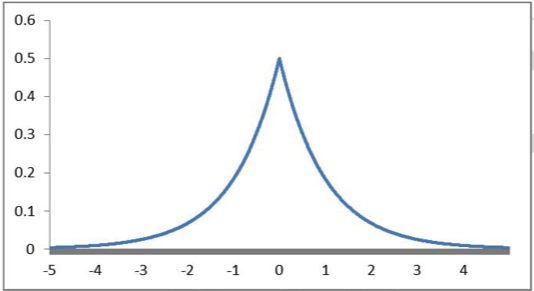
\includegraphics[width=0.6\textwidth]{../images/laplace-distribution.png}
	\caption{Laplace分布概率密度函数}
	\label{laplace-distribution}
\end{figure}

\paragraph{Laplace机制} Laplace机制仅适用于数值型结果的保护,通过向查询结果中加入服从Laplace分布的随机噪声来实现差分隐私保护。令设数据集D,函数f的敏感度为$\Delta f$,那么随机算法$M(D)=f(D)+Y$提供$\varepsilon$-差分隐私保护,其中$Y \sim Lap(\frac{\Delta f}{\varepsilon})$为随机噪声,服从尺度为$\frac{\Delta f}{\varepsilon}$的Laplace分布。

\paragraph{指数机制} 适用于非数值型查询结果。设随机算法M,输出为一实体对象$r \in Range$,函数$q(D,r)\rightarrow R $为可用性函数,$\Delta q$为函数$q(D,r)$的敏感度。若算法M以正比于$e^{\frac{\varepsilon q(D,r)}{2\Delta q}}$的概率从Range中选择并输出r,那么算法M提供$\varepsilon$-差分隐私保护。

\subsection{基于隐私保护的数据发布(PPDR)}
\paragraph{} PPDR研究的问题是如何在满足差分隐私的条件下保证发布数据或查询结果的精确性。根据实现环境可分为交互式数据发布和非交互式数据发布两种。
\subsubsection{交互式数据发布}
\paragraph{} “在交互式环境下,用户向数据管理者提出查询请求,数据管理者根据查询请求对数据集进行操作并将结果进行必要的干扰后反馈给用户,用户不能看到数据集全貌,从而保护数据集中的个体隐私”。具体可描述为:“给定数据集D和查询集合F,需寻求一种数据发布机制,使其能够在满足差分隐私保护的条件下逐个回答F中的查询,直到耗尽全部隐私保护预算”。“对于F中的任意f,设定一个足够小的实数$\delta$,查询结果精度$\alpha$应满足:
\begin{equation}
	Pr_{f\in F}[|f(D)-M(f(D))|\leq \alpha]\geq 1-\delta
\end{equation}
其中$f(D)$是查询结果,$M(f(D))$是对M的干扰结果。”
\subsubsection{非交互式数据发布} “在非交互式环境下,数据管理者针对所有可能的查询,在满足差分隐私的条件下一次性发布所有查询的结果。或者,数据管理者发布一个原始数据集的“净化”版本,这是一个不精确的数据集,用户可对该版本的数据集自行进行所需的查询操作”。可表述为:“给定D和F,需寻求一个数据发布机制,使其能够在满足差分隐私保护的条件下一次性回答F中所有的查询”。


\section{Privacy-preserving deep learning\cite{shokri2015ppdl}}
\subsection{Introduction}
\paragraph{} 本文提出一种协调深度学习系统,用于权衡效用和隐私。系统运行多方使用自己的输入数据合作训练一个神经网络模型,而不需要共享。此技术的关键创新是,在训练期间选择性共享模型参数。参数共享运行多个参与者在没有显式的输入数据的共享的情况下,互相利用其它人的模型计算结果。

\subsection{相关工作}
\subsubsection{Privacy in ML}
\paragraph{} 当多方利用自有数据协同执行机器学习任务时,基于安全多方计算(secure multi-party computation, SMC)的技术帮忙我们计算的中间步骤的隐私。

\subsection{Distributed Selective SGD}
\paragraph{} 本文方法的核心是分布式的、协作的深度学习协议,它基于以下观察结果:
\begin{itemize}
	\item 梯度下降的过程中,对不同参数的更新本质上是独立的;
	\item 不同的训练数据集作用于不同的参数;
	\item 不同的特征对目标函数的作用并不相等。
\end{itemize}
\paragraph{} 在进行选择性SGD时,学习器选择一部分参数进行更新,可选择梯度较大的那部分参数。
\subsection{系统架构}
\paragraph{概述} 系统由一个管理全局参数的参数服务器和多个局部训练器(参与者)组成,他们之间通过参数选择协议交换参数。参数交换协议允许参与者独立地优化参数、避免过拟合。
\paragraph{Local training} 每个参与者都可以在本地训练神经网络的参数。假设本地维护$w^{(i)}$个参数。训练过程如下:
\begin{enumerate}
	\item 将$\theta_d \times |w^{(i)}|$个参数下载并更新到本地,并不下载更新全部参数;
	\item 运行一轮SGD;
	\item 计算$\Delta w^{(i)}$,即新旧参数之间的差值;
	\item 选择性地上传最多$\theta_u \times |w^{(i)}|$个参数到服务器。选择方法有:
	\begin{itemize}
		\item 最大值选择:选择最大的几个值进行上传;
		\item 带阈值的随机选择:从大于阈值$\tau$的值中随机选择上传;
	\end{itemize}
\end{enumerate}
另外,上传$\Delta w^{(i)}$的值之前,这些值将被截断在$[-\gamma, \gamma]$之间,以避免这些值泄露训练数据的太多信息。
\paragraph{为什么DSSGD能行?} 这主要是因为学习过程的随机性。在训练过程中随机更新局部参数会增加局部SGD的随机性。而由异步参数更新导致的随机性对于精确地训练神经网络非常有效。
\paragraph{Parameter exchange protocol} 交换协议有三种类型:
\begin{itemize}
	\item 轮询。每个参与者按固定顺序下载、训练并更新一部分参数,然后下一个参与者继续;
	\item 随机。所有参与者同时随机下载、训练并更新一部分参数,但参数的读取过程是加锁的,也就是具有原则性(atomic);
	\item 异步。同随机一样,但并不加锁。
\end{itemize}
\subsection{Evaluation}
\paragraph{数据集} 实验选用的数据集是MNIST和SVHN
\paragraph{神经网络架构} 分别采用MLP和CNN
\paragraph{实验设置} 
\paragraph{选择性SGD的实验结果} SSGD的实验得到了以下结论:
\begin{itemize}
	\item SSGD可以获得与SGD相同的精度;
	\item SGD和SSGD在总体上是类似的;
	\item SSGD甚至能够取得比SGD更高的精度,这是因为SSGD类似于给SGD加上了Dropout。
\end{itemize}
\paragraph{DSSGD的实验结果} 结果表明:
\begin{itemize}
	\item 任何形式的协作都可以获得比独立学习更高的精度;
	\item 参与者的数量比共享参数的比例对精度的影响更小。
\end{itemize}
\subsection{Privacy}
\subsubsection{防止直接泄露}
\paragraph{训练过程} 在此过程中,由于各自的数据都不共享,所以不存在泄露。
\paragraph{模型使用过程} 此过程中也不需要使用到训练数据,因此也不存在泄露。

\subsubsection{防止间接泄露}

\section{Deep learning with differential privacy\cite{abadi2016deep} }
\subsection{Introduction}
\paragraph{} 深度学习模型不应该暴露数据集中的隐私信息,出于这个考虑,本文提出了一种学习算法,以较小的隐私预算训练非凸、规模巨大的深度网络。
\subsection{Our Approach}
\subsubsection{差分隐私SGD算法}
\paragraph{} 保护SGD过程中的隐私,其实就是对梯度进行隐私保护。本文的方法是首先根据限界对梯度进行修剪,然后再加上噪声。算法如下。
\paragraph{Norm clipping} 由于并没有关于梯度大小的先验界限,因此算法中使用$L_2$范数进行修剪。在算法中,如果$\left \| g \right \|_2 \leq C$,则g将被保护,如果$\left \| g \right \|_2 > C$ 则g将会被范数C缩放。
\paragraph{Lots} 在训练时,一个数据集一般被分为不交叉的多个batch,而此处的lot则指的是每次从整个数据集中随机取L条数据,每条数据被取出的概率是$q=L/N$,类似于,batch是不放回抽样,lot是放回抽样。
\paragraph{Privacy accounting} 差分隐私SGD需要计算总体隐私成本,可利用隐私的组合性质逐个进行计算,最后再求和。
\paragraph{Moments accountant} 


\section{The algorithmic foundations of differential privacy\cite{dwork2014algorithmic}}
\subsection{Basic Terms}
\subsubsection{Formalizing differential privacy}

\paragraph{概率单纯形(Probability Simplex)} 离散集合B上的概率单纯形定义为:
\begin{equation}
	\Delta (B) = \left \{ x \in R^{|B|}: x_i \geq \mbox{0 for all i and } \sum_{i=1}^{|B|} x_i=1 \right \}
\end{equation}
它是一个向量集合,其元素是一个概率表,一个|B|维向量,此向量每个元素代表一个概率,所有元素之和为1。
\paragraph{随机算法(Randomized Algorithm)} 定义域为A,值域为B的概率算法与一个映射$M:A \rightarrow \Delta (B)$相关联,对算法的输入$a \in A $,其输入为 $b \in B$,b的值是一个随机变量,满足分布$M(a)$。
\paragraph{隐私损失(Privacy loss)} 观察$\xi$引起的隐私损失定义为:
\begin{equation}
	L^{(\xi)}_{M(x)||X(y)}=ln(\frac{Pr[M(x)=\xi]}{Pr[M(y)=\xi]} )
\end{equation}
此值若为正,则说明一个观察结果更可以由x引起,若为负,则说明结果更可能由y引起。($\epsilon, \xi$)-差分隐私可以确保,对于所有的邻接集合x,y,隐私损失的绝对值都至少以概率$1-\delta$被限制在$\epsilon$ 以内。








\bibliographystyle{ieeepes}
\bibliography{../Saliency}
\end{document}